\documentclass[paper=a4, fontsize=11pt]{scrartcl} % A4 paper and 11pt font size

\usepackage[english]{babel} % English language/hyphenation
\usepackage{amsmath,amsfonts,amsthm} % Math packages
\usepackage{sectsty} % Allows customizing section commands
\allsectionsfont{\centering \normalfont\scshape} % Make all sections centered, the default font and small caps

\usepackage{fancyhdr} % Custom headers and footers
\usepackage{bm}
\usepackage{upgreek}
\usepackage{tikz}
\usetikzlibrary{shapes, arrows}

\pagestyle{fancyplain} % Makes all pages in the document conform to the custom headers and footers
\fancyhead{} % No page header - if you want one, create it in the same way as the footers below
\fancyfoot[L]{} % Empty left footer
\fancyfoot[C]{} % Empty center footer
\fancyfoot[R]{\thepage} % Page numbering for right footer
\renewcommand{\headrulewidth}{0pt} % Remove header underlines
\renewcommand{\footrulewidth}{0pt} % Remove footer underlines
\setlength{\headheight}{13.6pt} % Customize the height of the header

%-------------------------------
%	TITLE SECTION
%-------------------------------

\newcommand{\horrule}[1]{\rule{\linewidth}{#1}} % Create horizontal rule command with 1 argument of height

\title{
\normalfont \normalsize
\textsc{Brigham Young University} \\ [25pt] % Your university, school and/or department name(s)
\horrule{0.5pt} \\[0.4cm] % Thin top horizontal rule
\huge Practical High Speed Obstacle Avoidance in Unmanned Aerial Vehicles\\ % The assignment title
\horrule{2pt} \\[0.5cm] % Thick bottom horizontal rule
}

\author{James Jackson% <-this % stops a space
\thanks{James Jackson is with the Department of Mechanical Engineering, Brigham Young University
        {\tt\small jamesjackson@byu.edu}}%
        , Robert Pottorff
\thanks{Robert Pottorff is with the Department of Computer Science, Brigham Young University
        {\tt\small rpottorff@gmail.com}}%
}

\date{\normalsize\today} % Today's date or a custom date

\begin{document}

\maketitle % Print the title

% \abstract{Practical applications of UAVs are often limited by their ability to react to obstacles at high speeds. Although much progress has been made over the last few decades, current obstacle avoidance methods are either too slow or rely on unreasonable assumptions for some high-speed applications. Leaning on incredible recent successes applying deep reinforcement learning to high dimensional tasks, our agent consists of a deep actor-critic neural network trained using a combination of supervised and reinforcement learning techniques. We successfully control an agent that can fly up to 72km/h over various simulated obstacle-ridden terrain using only raw sensor data as input. Using inter-network statistics as a component of the cost function, we also demonstrate the successful transfer of learning from networks trained on simulated data, to agents running on real-world data and thereby achieve state-of-the-art results in real-world trials.}

\section{Introduction}

\begin{itemize}
	\item Why obstacle avoidance?
	\begin{itemize}
		\item Obstacle avoidance is an essential component of a safe operation of an autonomous agent.
		\item At high speeds obstacle avoidance is hard, and hasn't worked well so far
	\end{itemize}

	\item CS approach to Obstacle Avoidance
	\begin{itemize}
		\item Obstacle avoidance is a mapping of a sequence of sensor inputs to an action space
		\item Considering all the sensor data available at high speeds is intractable, but could become tractable given good abstraction
		\item What is the correct high-level space to appropriately handle obstacle avoidance?
	\end{itemize}
		
	\item Traditional Approach to Obstacle Avoidance
	\begin{itemize}
		\item Historically, most obstacle avoidance algorithms have relied on hand-crafted, closed-form rules applied to hand-picked transformations of the sensor space such as SIFT \cite{lowe1999object}, SURF \cite{bay2006surf}, or ORB key points \cite{rublee2011orb}
		\item These methods use key points to transform sensor data into a 3-dimensional models and optimize potential trajectories to minimize likelihood of collision
		\item Some methods have leveraged recent work in deep learning to minimize error between expert data and model data.
		\item Few of these methods have shown robustness to sensor choice, particularly at high speeds, and none, to our knowledge, have studied the impact of specialized high level abstractions learned exclusively for obstacle avoidance.
	\end{itemize}

	\item How to apply reinforcement learning to Obstacle Avoidance
	\begin{itemize}	
		\item Our motivation in this work is to show that the right high-dimensional feature space can enable an agent to perform with greater accuracy and at higher speeds than previous methods.
		\item We apply advancements made in reinforcement learning to actively learn high-level representations that maximize performance on obstacle avoidance tasks, enabling us to achieve state-of-the-art performance at high speeds in simulated worlds that can successfully transfer to real-world scenarios.
		\item The success of reinforcement learning to this domain points the way to a generalized algorithm for high speed control that is robust to sensor choice.
	\end{itemize}

	\item Motivate Transfer learning applied to Obstacle Avoidance
	\begin{itemize}
		\item Critical to reinforcement learning methods is the capacity to learn via trial and error, often a serious problem for real-world agents where failure is catastrophic.
		\item To overcome this problem, we also introduce a method for combining real world and simulated data.
		\item The success of reinforcement learning to this domain points the way to a generalized algorithm for high speed control that is robust to sensor choice.
	\end{itemize}

\end{itemize}

\section{Background}

\begin{itemize}
\item Traditional Obstacle Avoidance
	\begin{itemize}
		\item Most obstacle avoidance algorithms have focused on designing a closed-form avoidance rule given specific inputs.
		\item FFLOA~\cite{Scherer2007} - first ROAP, uses a heavy, specialized sensor, awesome results.
		\item Schopferer~\cite{Schopferer2014} - closest to optimal ROAP.  Considers kinematic feasibility of avoidance - What sensor did it use?
		\item Oleynikova~\cite{Oleynikova2015} - Stereo vision FFLOA
		\item Saunders~\cite{Saunders2009} - Local memory Voxel Grid-based planning
		\item Richter et al.~\cite{Richter2014} - Path planning based on learned probabilities of collision and optimizing a dynamic model
		\item Jackson~\cite{CEPA} - aimed at reducing limitations imposed by traditional algorithms
		\item none of these algorithms are fast enough to navigate a forest at 72km/h
		\item Expensive map creation
		\item dependence on SLAM
		\item assume nominal forward velocity
	\end{itemize}

\item  Reinforcement Learning
	\begin{itemize}
		\item reinforcement learning is the process of learning a control policy for an agent using a reward signal
		\item this is in contrast to supervised learning where a function is approximated using pairs of input and output signals
		\item reinforcement learning allows agents to be trained on environments in which there is no expert pilot data available
		\item it also allows agents to improve themselves over their lifetime \cite{thrun1995lifelong}

		\item formally reinforcement learning can be constructed as maximizing discounted total future reward over the execution of the policy
		\item \[math\]
		\item optimal action-value functions follow the form of Bellman equation
		\item \[math\]
		\item generally, reinforcement learning algorithms estimate $Q*$ using iterative update [math] \cite{Sutton:1998:IRL:551283}
		\item this is impractical for high dimensional feature spaces, so recently deep neural networks have been used to approximate $Q*$ \cite{Mnih2013}
		\item other applications of reinforcement learning to robotic motion in \cite{DBLP:conf/icra/KohlS04,DBLP:conf/iros/TedrakeZS04,geng2005fast,bagnell2001autonomous, riedmiller2009reinforcement}
		\item a more complete survey of reinforcement learning in robotics can be seen in \cite{kober2013reinforcement}
	\end{itemize}

\item Deep Neural Networks
	\begin{itemize}
		\item neural networks are a general function approximator that use alternating layers of linear and non-linear operations with parameters that are optimized with respect to a cost function
		\item in context of obstacle avoidance, neural networks have been used in ALVINN \cite{Pomerleau1989,Michels2005,riedmiller2009reinforcement}
		\item recently, a special type of neural network called a convolutional neural networks \cite{DBLP:journals/corr/SzegedyLJSRAEVR14} has vastly improved performance in many vision-based tasks
		\item convolutional neural networks have layers that convolve learned filters across the input producing spatially-aware activations
		\item because of their success, convnets are extremely common in vision applications
		\item pertinent applications to obstacle avoidance include classifying obstacles \cite{Hadsell2009}
		\item and supervised learning to map images to action spaces decided by an expert pilot \cite{Kim2015,Ross2013}
		\item most recently, \cite{Guisti2016} could follow an unknown trail in a forested area by training a DNN to minimize control error relative to an expert data set
		\item in our work, we use DNNs to approximate directly a mapping from sensor input to actions that avoids obstacles while on course to a target
		\item we train this network using reinforcement learning
	\end{itemize}

\item Transfer Learning
	\begin{itemize}
		\item Deep learning has so many parameters, needs tons of data AND reinforcement learning needs examples of failure therefore simulation is practically only option
		\item Simulation is cheap, but comes at the expense of realism
		\item Transferring from simulation to real-life is difficult
		\item transfer learning is the process of transferring knowledge embedded in one network into another network
		\item in our case we want to transfer learning from simulation to the real world
		\item in contrast to \cite{Michels2005} which simply constructs an ensemble of networks trained on different input spaces, true transfer learning augments a target with knowledge embedded from a source.
		\item this vastly improves performance as parameters can be tuned to minimize error in the target input space in a way that leverages data from both source and target network tasks
		\item recent work has been done with policy distillation \cite{Rusu2015} and progressive networks \cite{Rusu2016} to transfer policies between networks
		\item A new method, which we introduce here, applies techniques originally developed for style transfer to agent policy~\cite{Gatys2015}
	\end{itemize}

\item Application of Style Transfer to Policy Transfer
	\begin{itemize}
		\item recent work has shown gram matrices to be an effective way of capturing style of images \cite{Gatys2015}
		\item style transfer works by looking at the inner product of all neurons, and adding an addition component to the cost function
		\item \[math\]
		\item we apply a similar technique to transfer high-level abstractions learned in simulation to networks trained with expert data
		\item we do this by treating networks trained on simulated data as a source network, and networks trained on real data as a target network
		\item the additional constraint added during the training of the target network and is defined by the difference in the gram matrices between
		\item the two networks given the same input image
		\item \[math\]
		\item this constrains the manifold of target network parameters to a stricter subspace defined by the source network, accelerating learning
	\end{itemize}
\end{itemize}


\section{Approach} 
\begin{itemize}
	\item From a high level, we construct two simulators
	\item we train a combination of supervised and reinforcement learning on the first
	\item followed by fine-tuning using reinforcement learning in the second simulator
\end{itemize}

\begin{itemize}
	\item what is simulator A?
	\begin{itemize}
		\item built in gazebo
		\item obstacles are pylons and walls randomly placed (See Figure~\ref{fig:sample_environment})
		\item second order dynamics for pitch/roll/yaw
		\item first order dynamics for thrust
		\item collision calculation
		\item world is guaranteed to be traversable and meet constraints so that turning radius at n mph is at least x, and \cite{Richter2014}-like 
		\begin{figure}
		  \centering
		  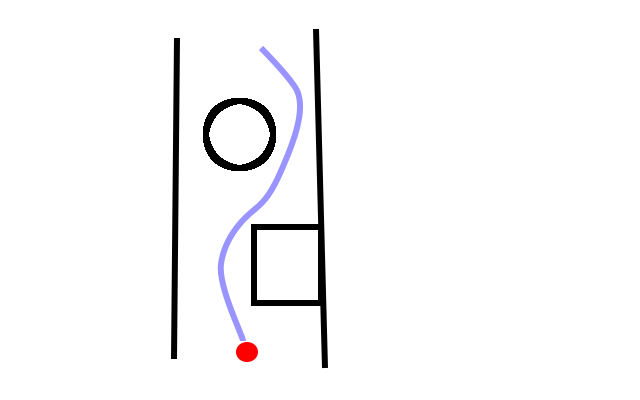
\includegraphics[width=0.5\textwidth]{fig/sample_environment.png}
		  \caption{Sample Simulated Environment}
		  \label{fig:sample_environment}
		\end{figure}
	\end{itemize}

	\item what is simulator B?
	\begin{itemize}
		\item same as A, but higher fidelity and slower
		\item obstacles are simulated to look like indoor cluttered environments
	\end{itemize}

	\item what does our network look like?
	\begin{itemize}
		\item identical structure to \cite{Lillicrap2015} using additional techniques of prioritized replay [citation needed], etc.
		\item hyper-parameters
		\item topology
		\item picture
	\end{itemize}

	\item how do we train an agent to succeed in supervised simulator A?
	\begin{itemize}
		\item similar to \cite{Kim2015} except with RRT in lieu of expert pilot 
		\item generate 10m training tuples of (sensor, goal trajectory, expected avoidance trajectory) over 10m (world, optimal trajectory)
		\item account for orientation bias in training tuples and real-life noise in sensor data
		\item cost function
		\item network details
	\end{itemize}

	\item how do we train an agent to succeed in unsupervised (RL) simulator A?
	\begin{itemize}
		\item similar to \cite{Lillicrap2015} except with pre-trained network and UAV task instead of whatever they use
		\item new worlds generated every episode similar to supervised worlds
		\item cost function / q learning math
		\item terminal state is defined as 5 meter radius to goal
		\item discretized reward every 10 meters vs change in inverse distance
		\item why discretized reward?
		\item negative reward on crash / death
	\end{itemize}

	\item how do we transfer knowledge from network A to network B
	\begin{itemize}
		\item network A (trained for simulation) has identical structure to network B (trained for real-world)
		\item train network A using simulation
		\item gather data for network B
		\item train network B with additional cost of minimizing gram matrix similarity
	\end{itemize}

\end{itemize}


\section{Results}

\begin{itemize}
	\item Simulator A Results
	\begin{itemize}
		\item How well does the network perform after supervised learning perform? (See Figure~\ref{fig:prob_completion_vs_epoch})
		\item How well does the network perform after reinforcement learning? See figure~\ref{fig:prob_completion_vs_epoch}
		\item How well does sup+reinforce work? See figure~\ref{fig:prob_completion_vs_epoch}
		\begin{figure}
		  \centering
			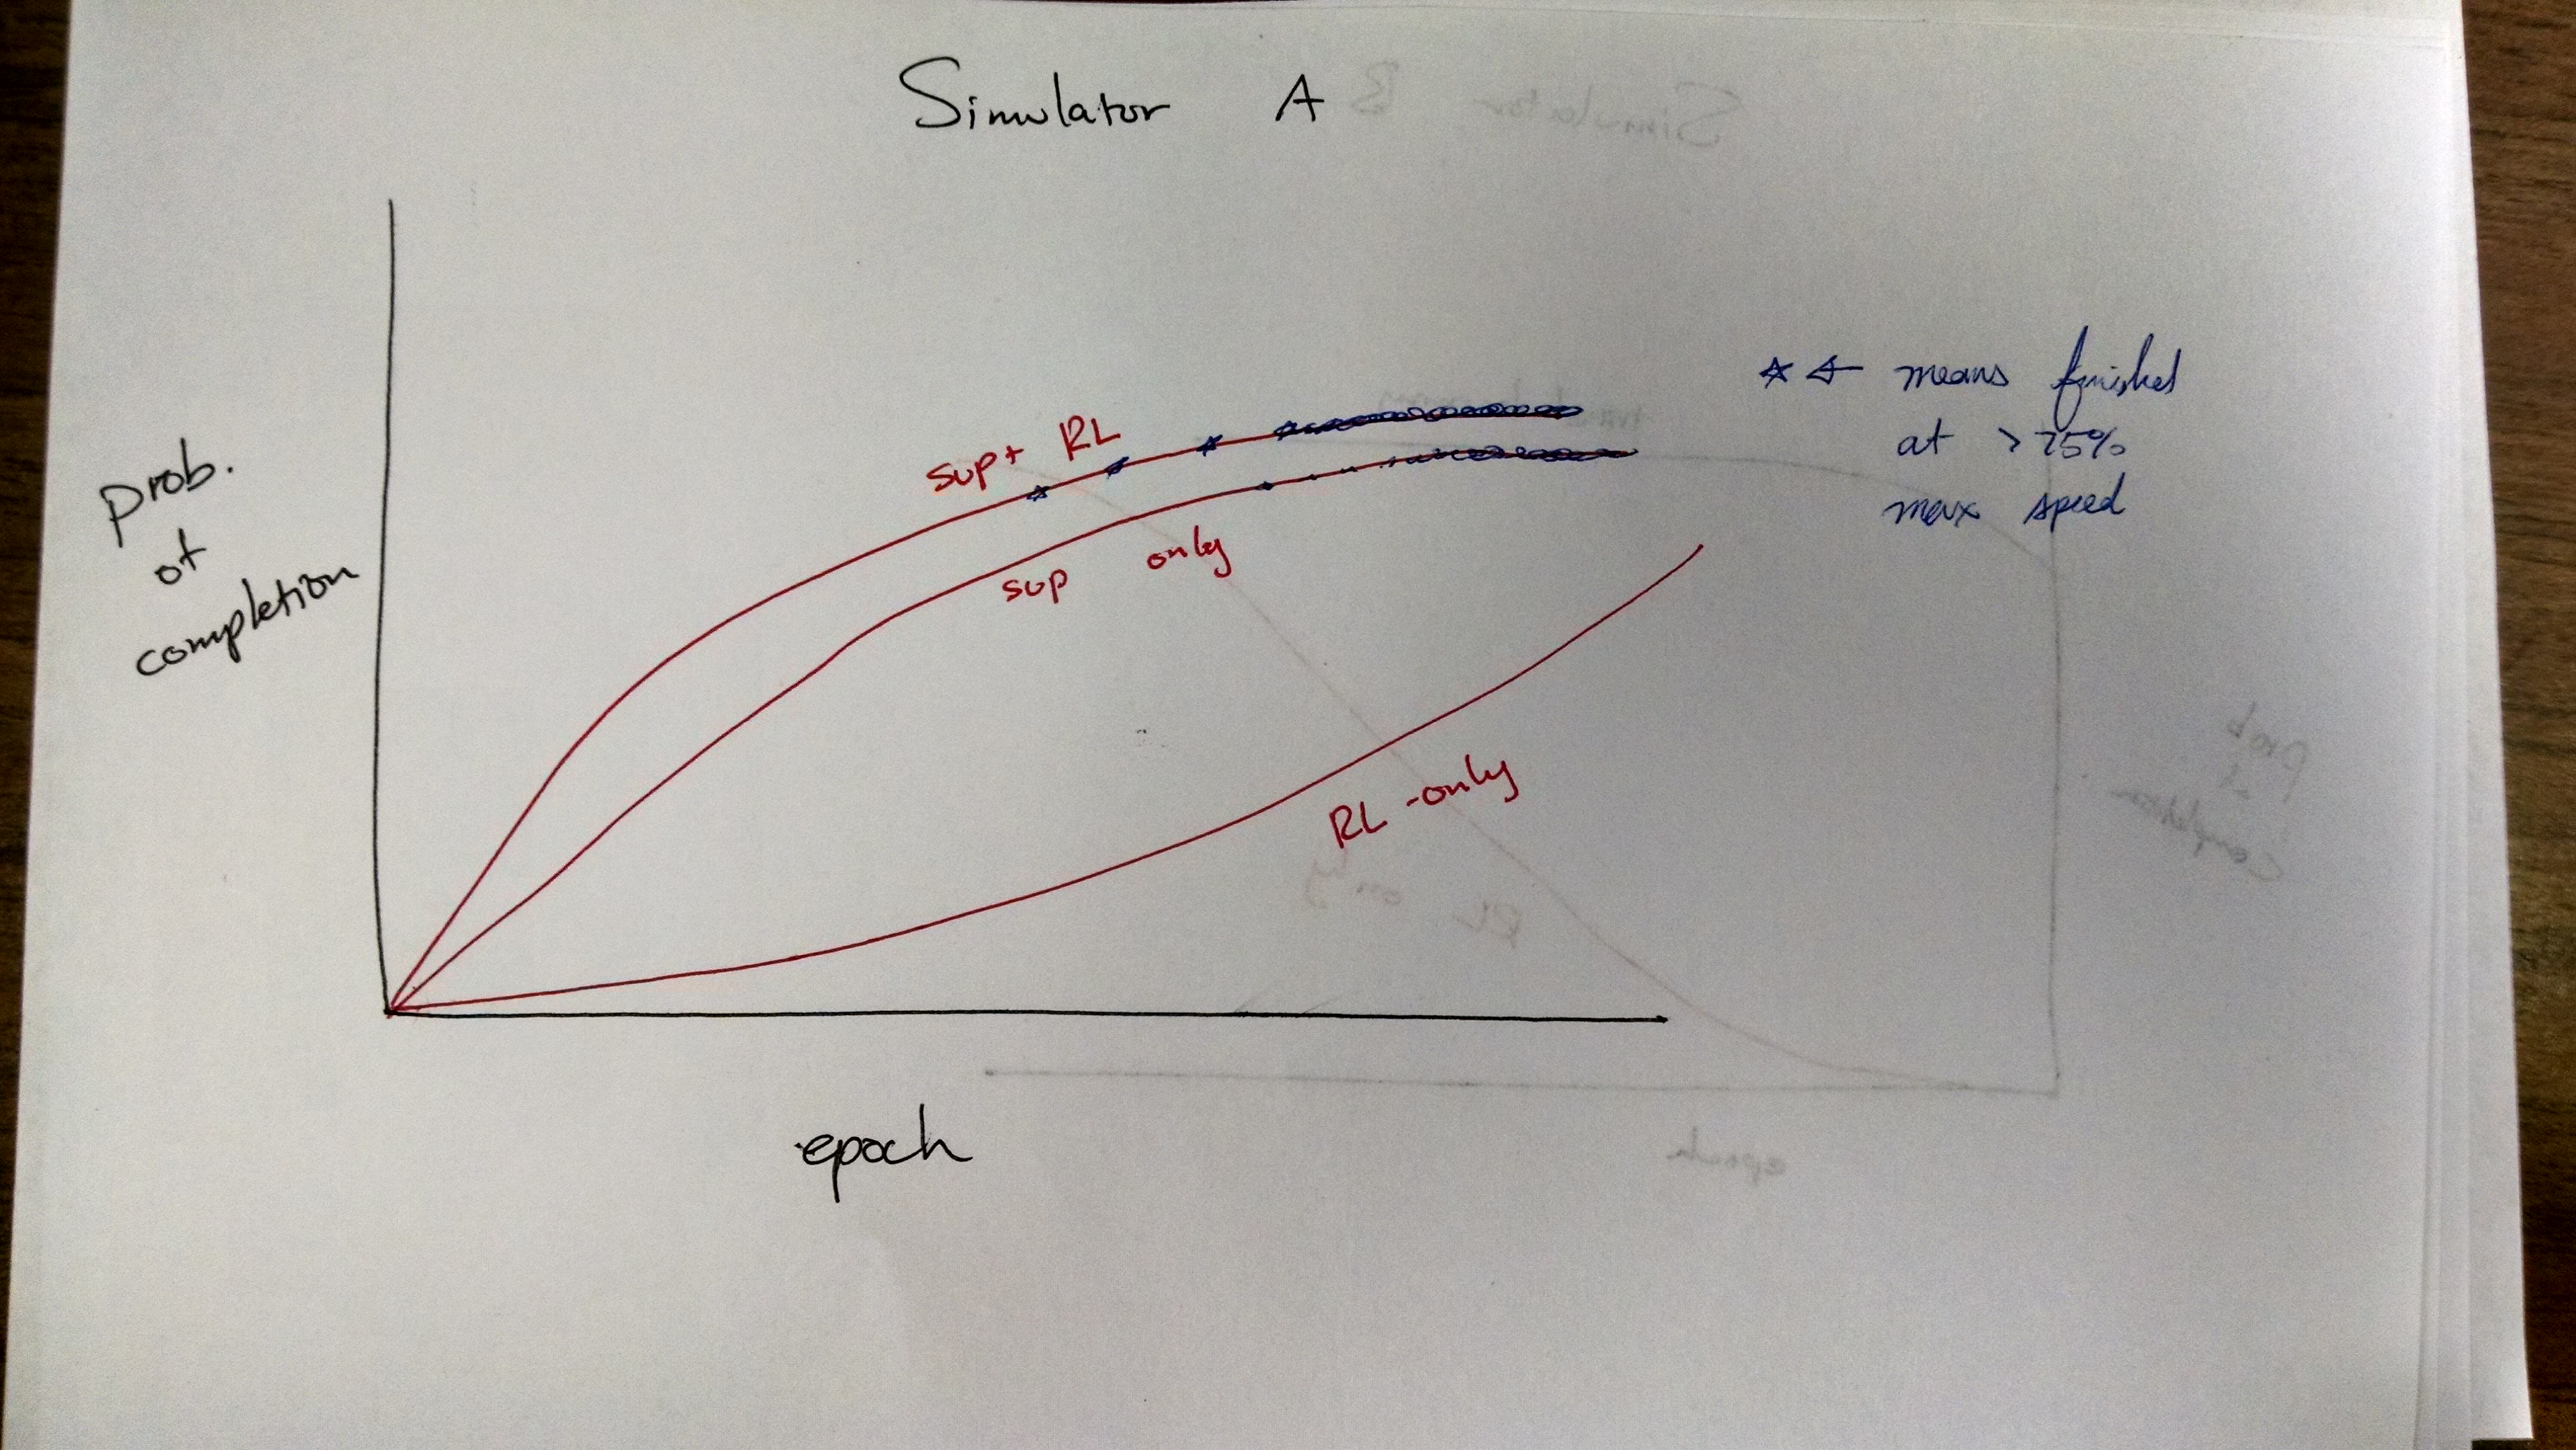
\includegraphics[width=0.5\textwidth]{fig/prob_of_completion_vs_epoch.jpg}
			\caption{probability of completion versus training epoch}
			\label{fig:prob_completion_vs_epoch}
		\end{figure}
	\end{itemize}

	\item Transfer Learning
	\begin{itemize}
	    \item What was the impact of the Reinforcement learning phase of Simulator B after transfer? (See Figure~\ref{fig:transfer_learning_vs_RL_sim_B})
		\item how many fewer epochs were required with transferred learning?
		\item Convolution Filters Between Networks (See Figure~\ref{fig:filter_comparison})
		\item How similar are the policies?  What are the differences? (See Figure~\ref{fig:policy_difference})
		\item Compare style transfer to Policy Distillation and Progressive Networks
		\begin{figure}
		  \centering
		  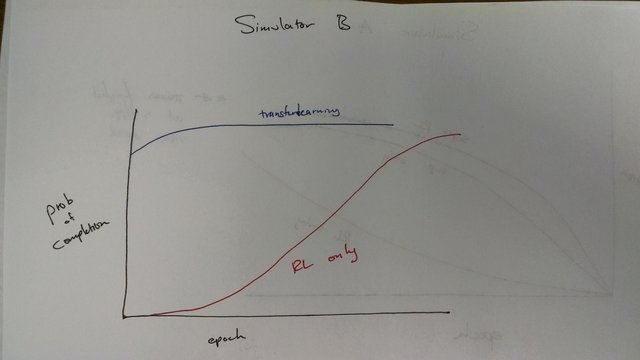
\includegraphics[width=0.5\textwidth]{fig/transfer_learning_vs_RL_sim_B.jpg}
		  \caption{Probability of Completion for the network using style transfer verses a standard reinforcement learner.  The network using transfer learning did better}
		  \label{fig:transfer_learning_vs_RL_sim_B}
		\end{figure}

		\begin{figure}
		  \centering
		  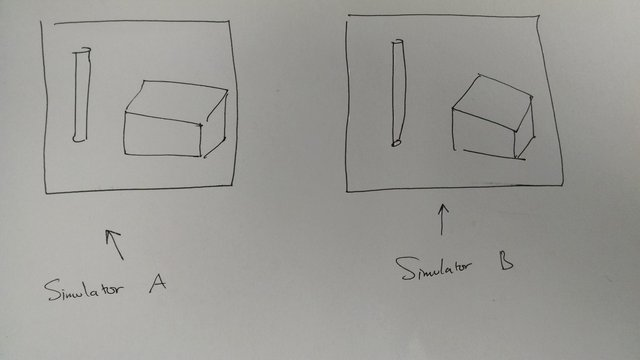
\includegraphics[width=0.5\textwidth]{fig/policy_difference.jpg}
		  \caption{Difference in policy between network trained in Simulator A vs Simulator B}
		  \label{fig:policy_difference}
		\end{figure}

		\begin{figure}
		  \centering
		  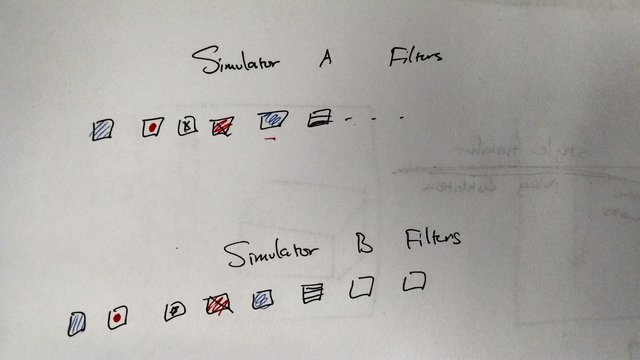
\includegraphics[width=0.5\textwidth]{fig/filter_comparison.jpg}
		  \caption{Comparison of Convolutional Filters learned by network trained in Simulator A vs Simulator B}
		  \label{fig:filter_comparison}
		\end{figure}

		\begin{figure}
		  \centering
		  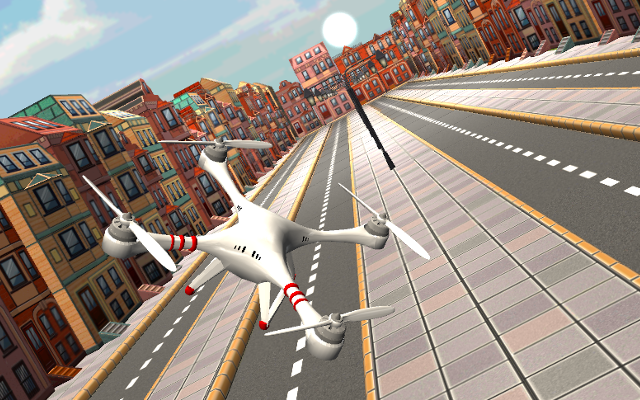
\includegraphics[width=0.5\textwidth]{fig/quadcopter_in_simulation.png}
		  \caption{Quadcopter in Simulation A}
		  \label{fig:sim_A}
		\end{figure}

		\begin{figure}
		  \centering
		  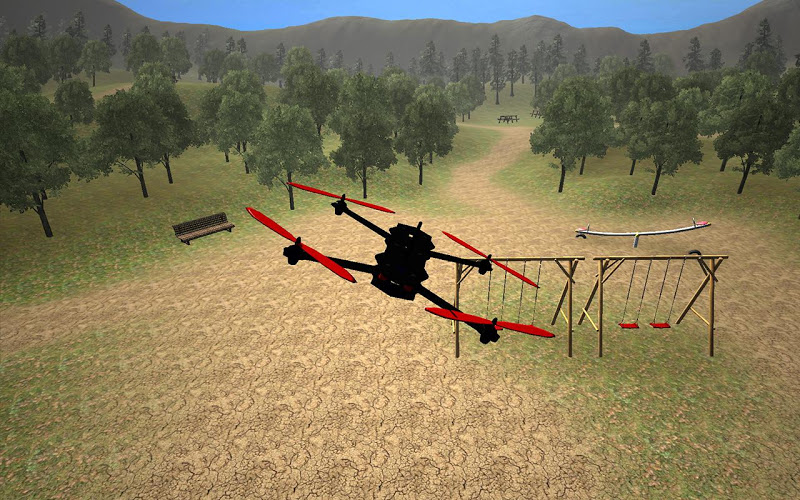
\includegraphics[width=0.5\textwidth]{fig/quadcopter_in_simulation_B.png}
		  \caption{Quadcopter in Simulation B}
		  \label{fig:sim_B}
		\end{figure}

	\end{itemize}

	\item Network Tuning
	\begin{itemize}
		\item What did we have to do to make the network learn?
		\item Comparison of Topologies
		\item Comparison of Hyper-Parameters
		\item Time to Convergence
	\end{itemize}

	\item Simulator B Results
	\begin{itemize}
		\item How well did it ultimately perform?
		\item Discussion of Speed (we went really fast)
	\end{itemize}

\end{itemize}

\section{Conclusion}

\begin{itemize}
	\item It works
	\item We went fast
	\item We learned some stuff about how style transfer can be used to transfer learning
	\item We learned how to transfer learning on robotic simulations
	\item We want to try it in real life
	\item There are other things we want to try too
\end{itemize}


\section{Appendix}


\bibliography{./library}
\bibliographystyle{plain}

\end{document}